The given information can be expressed as
    \begin{align}
    &\angle E= 60\degree=\theta \label{quad/43/eq1}
    \\
    &\angle A= 90\degree=\alpha \label{quad/43/eq2}
    \\
    &\norm{\vec{D}-\vec{E}} =4=a \label{quad/43/eq3}
    \\
    &\norm{\vec{E}-\vec{A}} =5=b \label{quad/43/eq4}
    \\
     &\norm{\vec{A}-\vec{R}} =4.5=c \label{quad/43/eq5}
    \end{align}
 Let, \begin{align}
    &\vec{E}=\myvec{0\\0}, \vec{A}=\myvec{5\\0}
\end{align}

\begin{lemma}
\label{quad/43/lemma}
\begin{align}
  & \vec{D} = a\vec{e}  \quad \brak{\because \vec{E}=\myvec{0\\0}} \label{quad/43/eq a}
\\
  & \vec{R} =\vec{A} + c\vec{a} \label{quad/43/eq b}
\end{align}
where 
\begin{align}
\vec{e} = \myvec{\cos E \\\sin E } ,\mathbf{a} = \myvec{\cos A\\\sin A }
\end{align}
\end{lemma}
Thus, 
from  \eqref{quad/43/eq1} and \eqref{quad/43/eq3} in \eqref{quad/43/eq a},
\begin{align}
\vec{D}&=4\myvec{\cos 60\degree \\\sin 60\degree }
\\
&=\myvec{2\\3.46}
\end{align}
and from \eqref{quad/43/eq2} and \eqref{quad/43/eq5} in \eqref{quad/43/eq b},
\begin{align}
\vec{R} &=\myvec{5\\0} + 4.5\myvec{\cos 90\degree \\\sin 90\degree }
\\
&=\myvec{5\\1}
\end{align}
Thus 
\begin{align}
 \vec{D}=\myvec{2\\3.46},\vec{E} = \myvec{0\\0}, \vec{A}=\myvec{5\\0},\vec{R}=\myvec{5\\1}
\end{align}
and the quadrilateral DEAR is the plotted in Fig. \ref{quad/43/fig:Quadrilateral DEAR}.	

\begin{figure}[!ht]
\centering
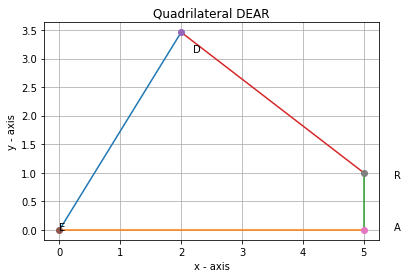
\includegraphics[ width=\columnwidth]{solutions/quad/43/download.png}
\caption{Quadrilateral DEAR}
\label{quad/43/fig:Quadrilateral DEAR}	
\end{figure}
